\documentclass[10pt,twocolumn,letterpaper]{article}

\usepackage{cvpr}
\usepackage{times}
\usepackage{epsfig}
\usepackage{graphicx}
\usepackage{amsmath}
\usepackage{amssymb}

\usepackage[ruled]{algorithm}
% \usepackage[options]{algorithm2e}
\usepackage{algpseudocode}
\usepackage{multirow}
\usepackage{booktabs}
\usepackage{subcaption}

% Include other packages here, before hyperref.

% If you comment hyperref and then uncomment it, you should delete
% egpaper.aux before re-running latex.  (Or just hit 'q' on the first latex
% run, let it finish, and you should be clear).
\usepackage[breaklinks=true,bookmarks=false]{hyperref}

\cvprfinalcopy % *** Uncomment this line for the final submission

\newcommand{\D}{\mathcal{D}}
\def\cvprPaperID{****} % *** Enter the CVPR Paper ID here
\def\httilde{\mbox{\tt\raisebox{-.5ex}{\symbol{126}}}}
\def\etal{\textit{et al.}}

% Pages are numbered in submission mode, and unnumbered in camera-ready
%\ifcvprfinal\pagestyle{empty}\fi
\setcounter{page}{1}
\begin{document}

%%%%%%%%% TITLE
\title{Class-wise Feature Distribution Matching Regularization\\ for Domain Generalization}

\author{Seungmin Lee\\
Seoul National University\\
{\tt\small profile2697@gmail.com}
% For a paper whose authors are all at the same institution,
% omit the following lines up until the closing ``}''.
% Additional authors and addresses can be added with ``\and'',
% just like the second author.
% To save space, use either the email address or home page, not both
}

\maketitle
%\thispagestyle{empty}

%%%%%%%%% ABSTRACT
\begin{abstract}
 Domain generalization (\textit{DG}) aims to learn a model that generalizes well to an unseen domain (\textit{target domain}), which has a different distribution than known domains (\textit{source domains}). Many of the previous works try to learn domain-invariant features. These methods adopt a loss that tries to match the whole distributions of the source domains. However, these works are sub-optimal because they rarely utilize task-specific information, such as class labels. Concerning the information, we propose a simple regularizing method called Class-wise Feature Distribution Matching (\textit{FDM}). The proposed method induces a model to produce similar features when the labels of examples are the same, regardless of the examples' domains. By doing this, the model is expected to learn more task-specific and invariant features than the previous works. To demonstrate the proposed methods, we conduct experiments on various settings. The proposed method consistently shows improvement compared to baseline. However, the improvement is marginal, and additional analysis reveals that domain-invariant features do not guarantee high performance.
\end{abstract}

%%%%%%%%% BODY TEXT
\section{Introduction}
Deep learning has been remarkably successful in many areas~\cite{}. However, many studies find out deep learning methods are hard to generalize when they encounter an unseen domain, which has a different data distribution than domains used for training~\cite{}. This problem called \textit{domain shift}~\cite{}. For alleviating the domain shift problem, some studies have been carried out on different assumptions. Domain Adaptation (DA) assumes there are two domains~\cite{}. The first is a fully-labeled source domain, and the other is a sparsely labeled or totally unlabeled target domain. Otherwise, domain generalization (DG) assumes there are some fully-labeled source domains, but the target domain is totally unavailable. DG is a challenge but an important research area because generalization to other domains is crucial to make a safe artificial intelligence. Moreover, it is helpful to understand how deep neural networks see the world.



\section{Related Works}
\subsection{Multi-Domain Learning and Multi-Source Domain Adaptation}
The primary purpose of Multi-Domain Learning (\textit{MDL}) is to learn a single model that can compactly represent all domains with a smaller number of parameters~\cite{yang2015mdlmtl, Rebuffi17, Bilen17, Rebuffi18}. For this purpose, Bilen~\etal~\cite{Bilen17} adopts shared model parameters except for batch normalization parameters and instance normalization parameters. Rebuffi~\etal~\cite{Rebuffi17} transforms the standard residual network architecture to share a significant amount of parameters between different domains.

Multi-Source Domain Adaptation (\textit{MSDA}) also uses a set of domains, but it additionally utilizes the images of an unlabeled target domain. The main focus of MSDA is to train a model that works well on the target domain without labels of it. Even though many studies have been conducted on single-source domain adaptation, there are a limited number of researches on MSDA~\cite{Zhao2018NIPS, Chang2019cvpr, guo2018-multi, peng2018moment}. Chang~\etal~\cite{Chang2019cvpr} proposes a domain-specific batch normalization with shared weights parameters and extends their method to MSDA. Peng~\etal~\cite{peng2018moment} suggests reducing moment distances between different domains. The moment distance measures the difference between feature distributions of two domains without concerning the task at hand.

MDL and MSDA are closely related to DG since DG also utilizes many sources in many cases. However, DG is different from MDL in that the primary focus of the DG is to learn semantic and domain-invariant features, not to learn compact representations. Moreover, DG is more challenging than MSDA because DG can not utilize the target domain in training.


\subsection{Domain Generalization}
Even though existing DG methods basically aim to learn domain-invariant features, these can be classified into several groups based on their strategies. The first group proposes a novel architecture~\cite{Khosla12undobias, Li2017dg}. The methods basically separate domain-specific parameters and domain-agnostic parameters. After that, they only extract and utilize the domain-agnostic parameters for the unseen domain. The second group of methods suggests optimization algorithms that adopt meta-learning or episodic learning~\cite{li2019episodic, Li2018MLDG, NIPS2018_metareg}. For example, MLDG~\cite{Li2018MLDG} constructs an episode by splitting the source domains into training domains and test domains in each iteration. The final group of methods uses losses that aims to learn domain-invariant features~\cite{Ghifary2015mtae, muandet2013domaingeneralization, mmdaaecvpr2018, carlucci2019domain}. The losses such as maximum mean distribution (\textit{MMD}) just try to match the feature distributions of all available source domains without concerning the task at hand. Therefore, methods that adopted MMD show sub-optimal performances~\cite{Saito2018, Saito2018b}. We propose a regularizing method using a simple consistency loss that explicitly utilizes the task-specific information. By using this simple loss, we expect that the model can learn domain-invariant but semantic features.

\section{Proposed Method}
\subsection{Problem Setting and Notation}
In DG, we assume that there are $n$ source domains $\D = \{\D_1, \D_2, \dots, \D_n\}$ where $\D_i$ indicates $i$-th source domain which contains sample-label pairs $\{x_i^j, y_i^j\}$. Using the source domains, our goal is to train a model $h$ that performs well on unseen target domain $\D_t$. We assume the model $h$ consists of a feature extractor $f$ and a classifier $c$. 

\subsection{Deep-All Method}
The Deep-All Method is a simple but effective baseline. In this method, we just aggregate all examples of source domains and train the model using the aggregated samples. If we work on a classification task, we can use cross-entropy loss as follows:
\begin{equation}
\label{eq:agg}
\begin{aligned}
L_{all} = \mathbb{E}_{\D_s\sim\D} \big[ \mathbb{E}_{\mathbf{x}_i,y_i\sim \mathcal{D}_s} \big[  {\mathbf{y}_i}^{T} \log h(\mathbf{x}_i) \big] \big]
\end{aligned}
\end{equation}
where $\mathbf{y}_i$ is a one-hot vector representation of $y_i$

\subsection{Class-wise Feature Distribution Matching Regularization}
We propose a consistency loss called Class-wise Feature Distribution Matching Regularization (\textit{FDM}), which tries to make a model generate similar features when the labels are the same. The FDM loss is calculated as follows: For each iteration, the feature extractor produces features of the source domains. After that, we calculate the averages of the features by classes. Lastly, the FDM loss is calculated as a consistency loss between the averages and the features that share the same label. The FDM loss is defined as follows:
\begin{equation}
\label{eq:fdm}
\begin{aligned}
L_{fdm} = \mathbb{E}_{\D_s\sim\D} \big[ \mathbb{E}_{\mathbf{x}_i,y_i\sim \mathcal{D}_s} \big[  \mathbb{D}_{KL}(f(\mathbf{x}_i)|| \mathbf{m}_{y_i}) \big] \big]
\end{aligned}
\end{equation}
where $\mathbb{D}_{KL}(\cdot || \cdot)$ represents Kullback–Leibler divergence and $\mathbf{m}_{y_i}$ is the average feature of class $y_i$. For simplicity, $\mathbf{m}_{y_i}$ is calculated for each batch. The $L_{fdm}$ regularize the feature extractor $f$ to extract similar features when the classes are the same.

Finally, overall loss function is defined as a weighted sum of $L_{all}$ and $L_{fdm}$ as follows:
\begin{equation}
\label{eq:overall}
\begin{aligned}
L = L_{all} + \lambda L_{fdm}
\end{aligned}
\end{equation}
where $\lambda$ is a hyperparameter that controlls the magnitude between the two losses.



\section{Experimental Results}
\subsection{Brief Summary of Datasets}
In this section, we give summaries of datasets used in our experiments. We use two different object classification datasets: \textbf{VLCS}~\cite{chen2013vlcs} and \textbf{PACS}~\cite{Li2017dg}. VLCS dataset consists of four famous datasets which are PASCAL VOC2007 (V)~\cite{Everingham10}, Labelme (L)~\cite{labelme}, Caltech 101 (C)~\cite{Feifei2004caltech}, and SUN09 (S)~\cite{Choi2010sun09}. Otherwise, PACS are composed of four datasets that have more significant visual domain gaps than those of VLCS. PACS consists of Photo (P), Art painting (A), Cartoon (C), and Sketch (S).

\subsection{Settings}
In this section, we evaluate the proposed method on standard DG benchmarks. For datasets, we use PACS~\cite{Li2017dg} and VLCS~\cite{chen2013vlcs}, which are commonly used for demonstrating DG algorithms. For networks, we adopt Alexnet~\cite{Krizhevsky2012} and ResNet-18~\cite{He2016resnet}. We found the architectures of Alexnet~\cite{Krizhevsky2012} used in each paper are different. Thus, we clarify the used structure in this paper is the same as Li~\etal~\cite{li2019episodic}. In each network, we use convolution layers as the feature extractor and fully-connected layers as the classifier. For hyperparameters, we set $\lambda_{max}$ to 0.1 and $T_r$ to 40 for all experiments. We train a model for 100 epochs and use the batch size 512 for all settings. Following the experiments' protocol used in Li~\etal~\cite{Li2017dg}, we evaluate the performance on a validation set during each epoch to get the best model, and we re-evaluate the performance on a test set using the model. We denote the proposed method as FDM in the results tables.


\subsection{Results on PACS + Alexnet}
The experimental results on PACS + Alexnet can be seen on Table~\ref{tab:pacs}. The proposed method shows a +1.7\% improvement compared to the Deep-All baseline, which indicates the proposed method could be helpful to DG tasks. Furthermore, In this setting, the proposed method shows better performance than the majority of the previous methods. Interestingly, the Deep-All baseline also exhibits better performance than many previous works, as mentioned in Li~\etal~\cite{li2019episodic}. Importantly, the proposed method shows better performance than all methods trying to match feature distribution without concerning the task at hand~\cite{ghifary2015domain, ganin2016dann, muandet2013domaingeneralization}. The proposed method also shows the best performance when the target domain is 'cartoon.'

\subsection{Results on VLCS + Alexnet}
To demonstrate the proposed method works well on another dataset, We evaluate FDM on VLCS + Alexnet. The results are on Table~\ref{tab:vlcs}. First, we could not reproduce the baseline of other works. Our baseline has almost 6\% lower performance than the Deep-All from Li~\etal~\cite{li2019episodic}. Therefore, we emphasize that the performance of our method has a large disadvantage than other methods in advance.  In this setting, FDM shows better performance than the baseline model. However, the gain is only +0.7\%, which is quite marginal. These results indicate the proposed regularization could be a hard constraint. We will discuss this problem at \ref{discussion}. Still, the proposed method shows better performance than ~\cite{lresvm, muandet2013domaingeneralization}. However, it shows weak performance than others. The disadvantage mentioned above seems to be a big cause, so it could not be fair comparisons.

\subsection{Results on PACS + ResNet-18}
We evaluate the proposed method on PACS + ResNet-18 to test whether FDM works well using different network architecture. The estimated results are on table~\ref{tab:pacs_resnet}. The proposed method consistently shows better performance than the Deep-All baseline. However, the gain is only +0.5\%, which indicates the proposed method can be redundant when the network structure is strong enough. Moreover, the proposed method only gives better performance than CrossGrad~\cite{shankar2018generalizing}. Nevertheless, the proposed method shows the best performance when the target domain is 'photo.' Interestingly, DANN~\cite{ganin2016dann} designed to match the feature distribution without concerning the task at hand also shows better performance than FDM and shows comparable performance than state-of-the-art methods. It indicates if the network is strong enough, and there is a set of source domains, a simple feature distribution matching would be enough. 

\begin{table*}[t]
	\centering
	\scalebox{0.7}{
		\begin{tabular}{cc|cccccccc|ccc}
			\toprule
			Src. & Trgt. & D-MTAE~\cite{Ghifary2015mtae} & LRE-SVM~\cite{lresvm} & CrossGrad~\cite{shankar2018generalizing} & DICA~\cite{muandet2013domaingeneralization}   &  DANN~\cite{ganin2016dann} & MetaReg~\cite{NIPS2018_metareg} & MLDG~\cite{Li2018MLDG} &  Epi-FCR~\cite{li2019episodic} & Deep-All (\cite{li2019episodic}) & Deep-All & FDM \\
			\midrule
			L,C,S&V& 63.9& 60.6 & 65.5 & 63.7& 66.4 & 65.0 & 67.7 & 67.1 & 65.4 & 59.7 & 59.3 \\
			V,C,S&L& 60.1& 59.7 & 60.0 & 58.2 & 64.0 & 60.2 & 61.3& 64.3 & 60.6 & 54.1 & 54.3\\
			V,L,S&C& 89.1 & 88.1 & 92.0 & 79.7 & 92.6&  92.3 & 94.4 & 94.1 & 93.1 & 87.7 & 88.0 \\
			V,L,C&S& 61.3& 54.9 & 64.7 & 61.0 & 63.6 & 64.2 & 65.9 & 65.9 & 65.8 & 61.4 & 64.0 \\
			\midrule
			\multicolumn{2}{c|}{Ave.}& 68.6 &65.8 &  70.5 & 65.7 & 71.7& 70.4 & 72.3 & 72.9 & 71.2 & 65.7 & 66.4\\
			\bottomrule
	\end{tabular}}
	\vspace{-0.2cm}
	\caption{\small Cross-domain object classification results (accuracy. \%) on VLCS using AlexNet.}
	% \vspace{-0.4cm}
	\label{tab:vlcs}
\end{table*}

\begin{table*}[t]
	\centering
	\scalebox{0.7}{
		\begin{tabular}{cc|ccccc|ccc}
			\toprule
			Src. & Trgt. & CrossGrad~\cite{shankar2018generalizing}&  DANN~\cite{ganin2016dann} & MetaReg~\cite{NIPS2018_metareg} & MLDG~\cite{Li2018MLDG} &  Epi-FCR~\cite{li2019episodic} & Deep-All & FDM \\
			\midrule
			P,C,S&A&  78.7 & 81.3 & 79.5& 79.5 & 82.1 &  77.3 & 77.7 \\
			P,A,S&C& 73.3 & 73.8 & 75.4&  77.3 & 77.0& 73.8 & 74.2\\
			A,C,S&P& 94.0 & 94.0& 94.3&  94.3 & 93.9 & 94.1 & 94.3 \\
			P,A,C&S& 65.1 & 74.3 & 72.2& 71.5 & 73.0 & 70.8 & 71.7 \\
			\midrule
			\multicolumn{2}{c|}{Ave.}& 77.8 & 80.8 & 80.4& 80.7& 81.5  & 79.0 & 79.5 \\
			\bottomrule
	\end{tabular}}
	\vspace{-0.3cm}
	\caption{\small Cross-domain object classification results (accuracy. \%) on PACS using ResNet-18.}
	\vspace{-0.4cm}
	% \vspace{-0.4cm}
	\label{tab:pacs_resnet}
\end{table*}

\section{Discussion}\label{discussion}
\subsection{Analysis: Hyperparameter Sensitivity}
For a further understanding of this work, we conduct hyperparameter sensitivity experiments on PACS + Alexnet. As in the previous experiment, we fix the value of $T_r$ at 40 for all tests. Instead, we experiment by changing the $\lambda_{max}$ value by 0.1, from 0 to 1. Note that $\lambda_{max} = 0$ is equivalent to the Deep-All baseline. The results are plotted in Fig.~\ref{fig:analysis}. The x-axis represents $\lambda_{max}$, and the left y-axis and the blue line denote the average L2 distance between the mean of representations of all examples and each example. We match the scale of the L2 distances by dividing the corresponding $\lambda_{max}$s. The right y-axis and the orange line represent mean accuracy on target domains. 

The proposed method only exceeds the baseline when the $\lambda_{max}$ is one of \{0.1, 0.2, 0.3\}. However, the difference between those three configurations is marginal, which means FDM is quite robust to hyperparameter in a small range. Nevertheless, the accuracies rapidly decrease when we use larger $\lambda_{max}$. The L2 distances gradually decrease as we increase the value of $\lambda_{max}$, which is quite natural. However, when we compare them with the distance of the baseline, the difference is more than x100. It indicates the proposed method provokes the network to produce domain-invariant features. Interestingly, the difference in corresponding accuracies is quite marginal. Therefore, we could infer that the domain-invariant features do not guarantee high performance, and the proposed method may be a too hard constraint.

\begin{figure}[t]
	\centering
	\footnotesize
	\begin{tabular}{c}
		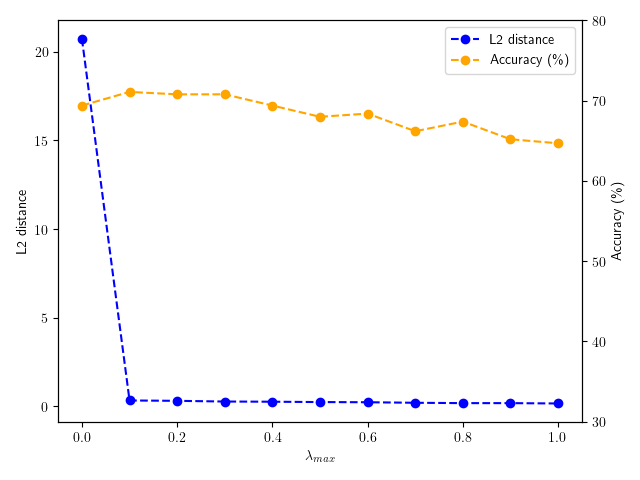
\includegraphics[width=8cm]{figures/analysis.png}
	\end{tabular}
	\vspace{-0.3cm}
	\caption{\textbf{The Plot of Hyperparameter Sensitivity on PACS + Alexnet} The orange line represents the mean accuracy of the four target domains. The blue line denotes the average L2 distance between the mean representation and the feature of each example.}\label{fig:analysis}
\end{figure}

\subsection{Why ResNet-18 Has a Smaller Gain Than Alexnet?}\label{resnet_discussion}
When we compare the performance gains of Alexnet (Table~\ref{tab:pacs}) and ResNet-18 (Table~\ref{tab:pacs_resnet}), we can see the performance gain in ResNet-18 is much smaller than that of Alexnet. It would indicate the redundancy of the proposed method. When we use the better architecture, the corresponding feature extractor would be able to extract discriminative features. \textbf{Those features may be variant in terms of distribution, but they could be considered invariant in terms of performing the task at hand.} Therefore, we need to design algorithms that can learn discriminative representations rather than trying to matching the feature distributions.




\section{Future Works}
We are planning to improve the proposed method further. According to the results, the proposed regularization seems too hard. Specifically, the proposed constraint prevents the model from learning more semantic features. Therefore, We are planning to find a way to soften or stabilize the regularization. Additionally, we will conduct more experiments and analysis using other datasets like VLCS~\cite{chen2013vlcs} and other models such as ResNet~\cite{He2016resnet}.

\section{Conclusion}
We suggest a simple regularization technique called Class-wise Feature Distribution Matching Regularization. We conduct various experiments to demonstrate the efficiency of the proposed method. The proposed method consistently improves the performance of the baseline. However, further analysis reveals that the domain-invariant achieved by the regularizing technique is not critical to the performance. Moreover, through the study, we could learn the invariant in terms of distribution is less important than the invariant regarding performing the task at hand.


{\small
\bibliographystyle{ieee_fullname}
\bibliography{egbib}
}

\end{document}
